\documentclass[border=1pt]{standalone}
\usepackage[dvipsnames]{xcolor}
\usepackage{tikz}                       % Graphen und kommutative Diagramme
\usetikzlibrary{patterns}               % Um schraffierte Formen in der tikzpicture-Umgebung zu zeichnen.
\newcommand{\ul}[1]{\underline{\smash{#1}}}
\begin{document}
\centering
\begin{minipage}{.55\textwidth}
    \centering
    \resizebox{\textwidth}{!}{
        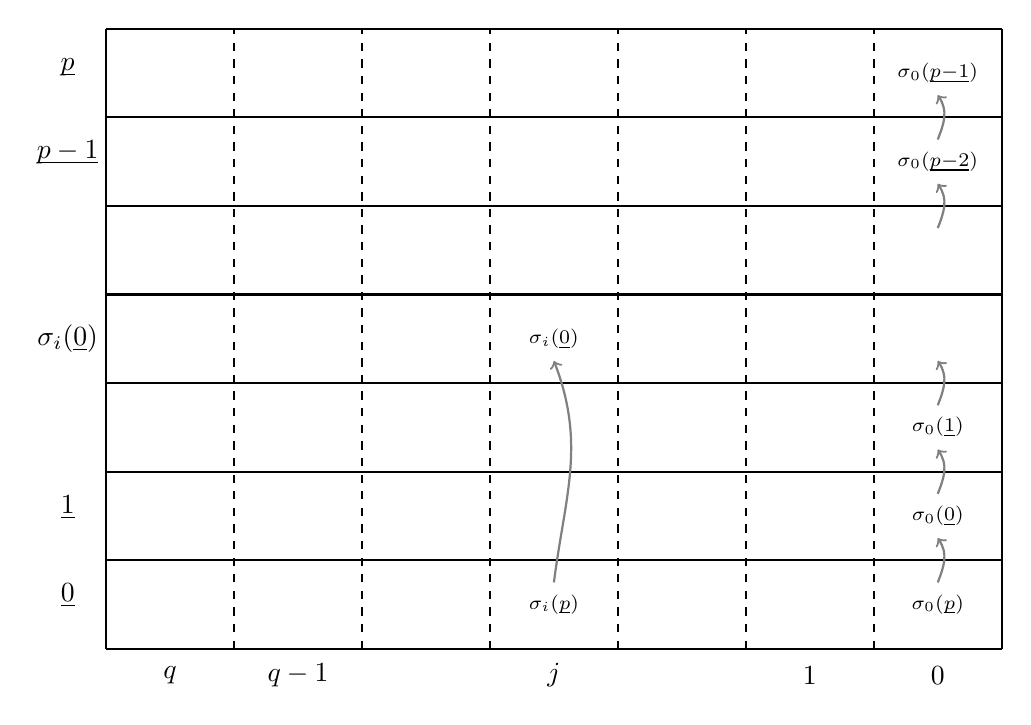
\begin{tikzpicture}[yscale=.9, xscale=1.3, x=1.25cm, y=1.25cm, line width=.8pt]
            % Linien.
            \foreach \i in {0,...,7}
            {
                \draw[color=black] (0,\i) -- (7,\i);
            }
            \draw[color=black] (0,0) -- (0,7);
            \draw[color=black] (7,0) -- (7,7);
            \foreach \i in {1,...,6}
            {
                \draw[color=black, dashed] (\i,0) -- (\i,7);
            }
            
            % Beschriftung.
            \draw node at (-.3,6.5) {$\ul p$};
            \draw node at (-.3,5.5) {$\ul {p-1}$};
            \draw node at (-.3,3.5) {$\sigma_i(\ul 0)$};
            \draw node at (-.3,1.5) {$\ul 1$};
            \draw node at (-.3,0.5) {$\ul 0$};
            
            \draw node at (0.5,-.3) {$q$};
            \draw node at (1.5,-.3) {${q-1}$};
            \draw node at (3.5,-.3) {$j$};
            \draw node at (5.5,-.3) {$1$};
            \draw node at (6.5,-.3) {$0$};
            
            \draw[->, color=black!50] (6.5, 0.75) to[out=75, in=295] (6.5, 1.25);
            \draw[->, color=black!50] (6.5, 1.75) to[out=75, in=295] (6.5, 2.25);
            \draw[->, color=black!50] (6.5, 2.75) to[out=75, in=295] (6.5, 3.25);
            \draw[->, color=black!50] (6.5, 4.75) to[out=75, in=295] (6.5, 5.25);
            \draw[->, color=black!50] (6.5, 5.75) to[out=75, in=295] (6.5, 6.25);
            
            \draw node at (6.5, 0.5) {$\scriptstyle \sigma_0(\ul p)$};
            \draw node at (6.5, 1.5) {$\scriptstyle \sigma_0(\ul 0)$};
            \draw node at (6.5, 2.5) {$\scriptstyle \sigma_0(\ul 1)$};
            \draw node at (6.5, 5.5) {$\scriptstyle \sigma_0(\ul {p-2})$};
            \draw node at (6.5, 6.5) {$\scriptstyle \sigma_0(\ul {p-1})$};
        %     
        %     \draw[->, color=black!50] (2.5, 0.75) to[out=85, in=285] (2.5, 5.25);
        %     \draw node at (2.5, 0.5) {$\scriptstyle \sigma_{i+1}(p)$};
        %     \draw node at (2.5, 5.5) {$\scriptstyle \sigma_{i+1}(0)$};
                
            \draw[->, color=black!50] (3.5, 0.75) to[out=85, in=285] (3.5, 3.25);
            \draw node at (3.5, 0.5) {$\scriptstyle \sigma_i(\ul p)$};
            \draw node at (3.5, 3.5) {$\scriptstyle \sigma_i(\ul 0)$};  
        \end{tikzpicture}
    }
\end{minipage}
\hspace{.4cm}
\begin{minipage}{.55\textwidth}
    \centering
    \resizebox{\textwidth}{!}{
        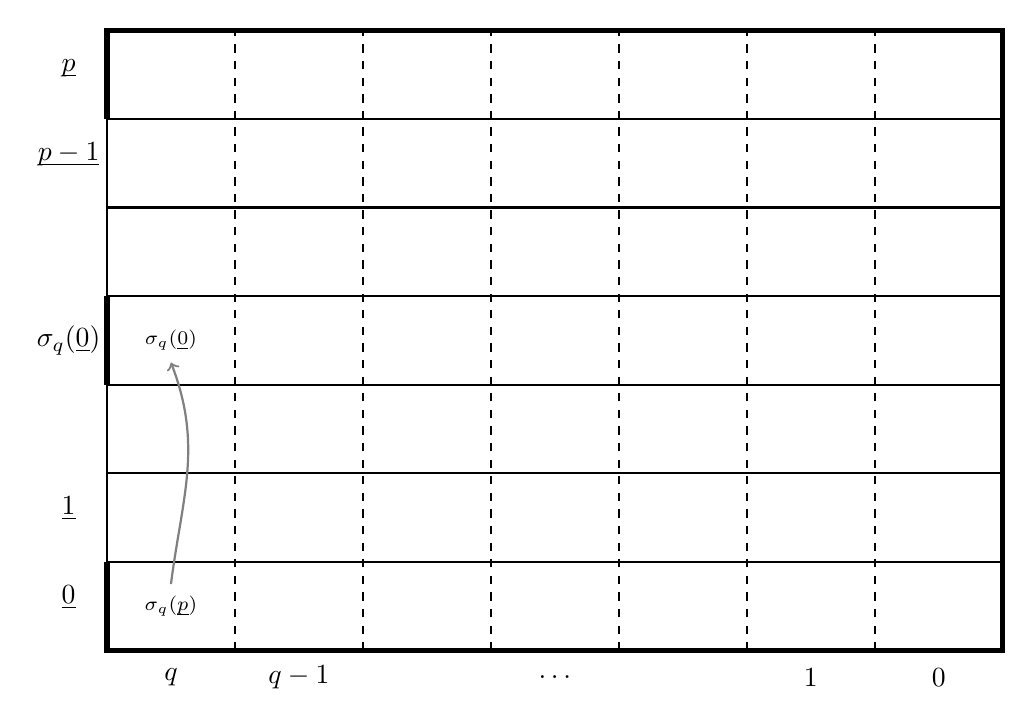
\begin{tikzpicture}[yscale=.9, xscale=1.3, x=1.25cm, y=1.25cm, line width=.8pt]
            % Linien.
            \foreach \i in {0,...,7}
            {-
                \draw[color=black] (0,\i) -- (7,\i);
            }
            \draw[color=black] (0,0) -- (0,7);
            \draw[color=black] (7,0) -- (7,7);
            \foreach \i in {1,...,6}
            {
                \draw[color=black, dashed] (\i,0) -- (\i,7);
            }
            
            \draw[color=black, line width=2pt] (0,1) -- (0,0) -- (7,0) -- (7,7) -- (0,7) -- (0,6);
            \draw[color=black, line width=2pt] (0,3) -- (0,4);
            
            \draw[->, color=black!50] (0.5, 0.75) to[out=85, in=285] (0.5, 3.25);
            \draw node at (0.5, 0.5) {$\scriptstyle \sigma_q(\ul p)$};
            \draw node at (0.5, 3.5) {$\scriptstyle \sigma_q(\ul 0)$};
            
            % Beschriftung.
            \draw node at (-.3,6.5) {$\ul p$};
            \draw node at (-.3,5.5) {$\ul {p-1}$};
            \draw node at (-.3,3.5) {$\sigma_q(\ul 0)$};
            \draw node at (-.3,1.5) {$\ul 1$};
            \draw node at (-.3,0.5) {$\ul 0$};
            
            \draw node at (0.5,-.3) {$q$};
            \draw node at (1.5,-.3) {$q-1$};
            \draw node at (3.5,-.3) {$\ldots$};
            \draw node at (5.5,-.3) {$1$};
            \draw node at (6.5,-.3) {$0$};
        \end{tikzpicture}
}
\end{minipage}
\end{document}